

\documentclass[pdftex,10pt,a4paper]{article}
%Can change the pt, papersize etc.

\usepackage{amsmath} %For both in-line and equation mode
\numberwithin{equation}{section} %Numbering of our equations per section
\usepackage{algorithm}
\usepackage{algorithmic} %Algorithm styles, need to be nested for the example shown
\usepackage{fancyhdr} %For our headers
\usepackage{graphicx} %Inserting images
\usepackage{lipsum}  %Blank text fill, delete me when finished
\usepackage{setspace} %Spacing on the front page for crest and titles
\usepackage[]{fncychap} % Styles can be Sonny, Lenny, Glenn, Conny, Rejne, Bjarne and Bjornstrup
\usepackage[hyphens]{url} %Deals with hyphens in urls to make them clickable
\usepackage{xcolor} %Great if you want coloured text
\usepackage{tabularx}
\usepackage{appendix} %Take a wild guess slick
\usepackage{amsmath, amssymb, amsthm}
\usepackage{wasysym}
\usepackage[export]{adjustbox}

%KEEP THIS ONE LAST it's quite buggy, it allows you to click on links within the pdf and web links without changing the colour. The mouse cursor simply changes its icon to indicate to the user. Great tool - still awkward
\usepackage[hidelinks]{hyperref}



%This will tell the compiler to do the header style, page and spacing between the header and text
\fancyhf{}
\pagestyle{fancy}
\renewcommand{\headrulewidth}{0.2pt}


\fancyhead[L]{Group 19}
\fancyhead[C]{CISC 204: Modelling Project (FINAL)}
\fancyhead[R]{Page \thepage}


%%%%%%%%%%%%%%%%%%%%%%%%%% DOCUMENT STARTS %%%%%%%%%%%%%%%%%%%%%%%%%%%%%


\newcommand{\groupid}{GRP\_123}
\newcommand{\projectname}{Project Name}


\newcommand{\authors}
{
Name of Teammate 1 (and their NetID)\\s
Name of Teammate 2 (and their NetID)\\
Name of Teammate 3 (and their NetID)\\
}



%Lets begin the document, some chapters have examples in to give you an idea 
\begin{document}

\tableofcontents

\section*{Summary}
\addcontentsline{toc}{section}{Summary}
% \vspace{2cm}
We are exploring the popular board game 'The Resistance' through a formal logic lens, where the turn-based format with 2 teams (Spies, Resistance) and hidden player identities allow the establishment of propositional models that are solvable by computer. The 7 players go on a series of 'missions' which are voted to go ahead or not by a subset of all players selected by a leader in each of the 5 rounds. A mission succeeds for the Resistance team and gains them a point if all participants submit a 'success' card in an anonymous choice procedure, which is the key game mechanic as a given player doesn't directly know the team membership of other players and is forced to infer this information as the rounds progress. Spies can submit a 'fail' card and cause the mission to fail which gives them one point, and either team wins the game with 3 points.

Implementation proved to be non-trivial due to assigning models encompassing all possible play combinations per round and evaluating their satisfiability. Critically, votes were assigned randomly to simulate player behaviour which enabled a method of calculating the likelihood of the Resistance team winning at each stage of the game, as suggested by Prof. Muise after the proposal to properly expand the scope of our project. 


\section*{Propositions}
\addcontentsline{toc}{section}{Propositions}
%List of the propositions used in the model, and their (English) interpretation.
$X_r$ is true at position $r$ depending on the round number (e.g. $X_2$ is true for r2)\newline
$Z_s$ is true if current mission is rejected $s$ times (e.g. $Z_3$ means the 3rd consecutive rejection) \newline
Note that $r$ and $s$ both range from 1 to 5, but $X_r$ and $Z_s$ don't necessarily have the same truth value when $r=s$ due to how the game functions\newline
$Y_k$ is true if mission $k$ is approved, false if not (e.g. $\neg Y_4$ means mission 4 not approved) \newline
$P_i$ is true if player $i$ has voted to approve the current mission and false otherwise, where $i$ ranges from 1 to 6 \newline
$Q_j$ is true if player $j$ has played a success token in the currently approved mission, false if player $j$ has played a fail token (e.g. $\neg Q_1$ means player 1 has played a fail token) \newline
Note that $i$ ranges from either 1 to 3 or 1 to 4 depending on the number of players per round \newline
$S_r$ is true if the current mission is a success for team Resistance and false otherwise, and vice-versa for team Spies \newline
$V$ represents the overall game victory condition: true for the Resistance winning the game, false for the Spies emerging victorious\newline

\section*{Constraints}
\addcontentsline{toc}{section}{Constrains}
%List of constraint types used in the model and their (English) interpretation. You only need to provide one example for each constraint type: e.g., if you have constraints saying “cars have one colour assigned” in a car configuration setting, then you only need to show the constraints for a single car. Essentially, we want to see the pattern for all of the types of constraints, and not every constraint enumerated.\newline

Detailed description of the game rules:

7 players total $\rightarrow$ 4 R, 3 S\newline
\indent 5 total rounds ('missions')$\rightarrow$ a team wins if they succeed in 3/5 in any order\newline

Round structure:

\indent r1: 3 players \newline
\indent	r2: 4 players \newline
\indent	r3: 3 players \newline
\indent	r4: 4 players \newline
\indent	r5: 4 players \newline


Before the game starts (i.e. r0) each player is randomly assigned a team which none of the other players know. This assignment lasts until the game ends.
At the start of each round, one player is assigned the role of 'mission leader' \& the remaining 6 are given 1 accept and 1 reject token for voting purposes. The leader then gets to choose the corresponding number of players per round from the pool to send on the mission as above (leader not included).\newline

Mission start:\newline \newline
\indent Selected players vote to either accept or reject the current mission. \newline
\indent If a majority reject the mission, then the next counterclockwise player is \indent assigned leader. NOTE: If 5 rejections occur in a row then the S team \indent wins automatically. The vote tracker resets every round (e.g. r2 can have 1 \indent rejection, r3 0, r4 3, etc.)\newline
\indent If a majority accept the mission, then each active player is given 1 success \indent card and 1 failure card. NOTE: R players have to play success every time, \indent whereas S players can play either success or failure. Once all players turn in \indent their cards then the total number is counted. If there's $\ge$1 fail cards then \indent the current mission fails $\rightarrow$ 1 point for team S. Otherwise, 1 point for team R \newline

\indent If there's a tie of accept/reject tokens (possible on rounds w/ an even \indent number of players) then flip a coin to see whether the mission happens or \indent not (H  yes, T no).\newline 

Mission end\newline

At the end of any round, if a team gets 3 points then they are declared the \indent winner, unless the above win condition for team S is satisfied. \newline

As per Prof. Moose's suggestion, we've expanded the scope of the constraints by imagining that at the time of player selection for each mission the leader will have access to a computer with the Python scripts for this project, and they will attempt to calculate an estimate of winning based on the probability that the other players are on team R or team S. This is done by simply counting the number of valid models (propositional formulas evaluating to true under the selected conditions) and dividing by the total number of models:

\begin{equation}
	P(win)=\frac{n_{valid}}{n_{valid} + n_{invalid}}
\end{equation} \newline

We proceed through an example game with specific votes \& tokens to illustrate how the constraints are expressed in propositional logic.\newline 

Round 1:\newline

$X_1 \land (\neg P_1 \land \neg P_2 \land P_3 \land \neg P_4 \land \neg P_5 \land P_6) \rightarrow \neg Y_1 \land Z_1$ \newline

Here 4/6 players voted to reject the mission so $Y_1, Z_1$ are updated. \newline \newline

$X_1 \land (P_1 \land \neg P_2 \land \neg P_3 \land \neg P_4 \land \neg P_5 \land \neg P_6) \rightarrow \neg Y_1 \land Z_1 \land Z_2$ \newline

Here 5/6 players voted to reject the mission, with $Z_2$ added accordingly.

...\newline
\indent Voting rounds 3 and 4 also result in rejections.\newline
\indent ...\newline

$X_1 \land (\neg P_1 \land \neg P_2 \land \neg P_3 \land \neg P_4 \land \neg P_5 \land \neg P_6) \rightarrow \neg Y_1 \land Z_1 \land Z_2 \land Z_3 \land Z_4 \land Z_5$ \newline
\indent $Z_5 \rightarrow \neg V$\newline

After 5 rejections, the Spies automatically win the game. \newline

Alternatively, let's say the 1st mission is approved:

$X_1 \land ( P_1 \land \neg P_2 \land P_3 \land P_4 \land \neg P_5 \land P_6) \rightarrow Y_1 $ \newline

Only 2/6 players voted against so now the mission can go ahead. \newline

$Y_1 \land ( Q_1 \land Q_2 \land Q_3) \rightarrow S_1 $\newline

\indent In this scenario round 1 counts as a success for the Resistance as none of the \indent players put forward a fail token.\newline

Round 2:

$X_2 \land ( P_1 \land P_2 \land P_3 \land \neg P_4 \land P_5 \land P_6) \rightarrow Y_2 $ \newline

$Y_2 \land ( \neg Q_1 \land Q_2 \land Q_3 \land \neg Q_4) \rightarrow \neg S_1 $\newline

Here the mission is approved right away, and Spies win the round by playing \indent a single failure token.\newline

Round 3:

$X_3 \land ( \neg P_1 \land \neg P_2 \land P_3 \land \neg P_4 \land P_5 \land \neg P_6) \rightarrow \neg Y_3 \land Z_1$ \newline

$X_3 \land ( P_1 \land P_2 \land P_3 \land \neg P_4 \land P_5 \land P_6) \rightarrow Y_3 \land Z_1 \land \neg Z_2$ \newline

Here the mission is approved on the 2nd voting round; notice how the $Z_s$ \indent counter resets to 1 at every round.\newline

$Y_3 \land ( \neg Q_1 \land Q_2 \land Q_3) \rightarrow  S_3 $\newline

The $Q_j$'s and $P_i$'s are also different per round. Here the Resistance wins \indent mission 3.\newline \newline
\indent...\newline
\indent Round 4 is a win for team Spies\newline
\indent...\newline


Round 5:\newline

$X_5 \land ( P_1 \land P_2 \land P_3 \land P_4 \land P_5 \land P_6) \rightarrow Y_5 $ \newline

$Y_5 \land (Q_1 \land Q_2 \land Q_3 \land Q_4) \rightarrow \neg S_5  $\newline

The final tally is then: \newline

$S_1 \land \neg S_2 \land S_3 \land \neg S_4 \land S_5 \rightarrow V $ \newline \newline \indent RESISTANCE WINS - YAHOO! \newline

Alternatively, let's assume that the Spies win in rounds 1, 2, and 4:\newline

$\neg S_1 \land \neg S_2 \land S_3 \land \neg S_4 \rightarrow \neg V $ \newline

In this case the Spies automatically win after round 4 finishes as they have \indent the required 3/5 missions. It's also possible for the Resistance to win after \indent having played only 3 rounds, etc.\newline

It's also possible to chain together a massive series of disjunctions for all the \indent winning combinations of $S_r$'s for the Resistance:

\begin{equation}
	(S_1 \land S_2 \land S_3 \land \neg S_4 \land S_5) \lor (\neg S_1 \land S_2 \land S_3 \land S_4 \land S_5) \lor ... \lor (S_1 \land S_2 \land \neg S_3 \land \neg S_4 \land S_5) \rightarrow V
\end{equation} \newline

In the same way we can list all the possibilities that lead to a victory for the \indent Spies. Bada-bing!

\section*{Jape Proofs}
\addcontentsline{toc}{section}{Jape Proofs}
Please see the attached file proofs.jp.\newline
We had trouble assigning subscripts, so the following images are for clarification purposes (variable names are different than in the Propositions section, i.e. $R_i=Q_j, S=S_r, Q=V$):\newline

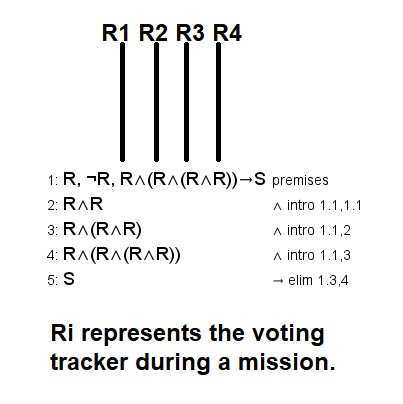
\includegraphics[scale=0.7]{im1.jpg}\newline
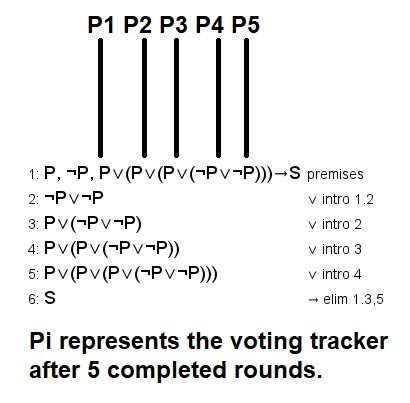
\includegraphics[scale=0.7]{im2.jpg}\newline
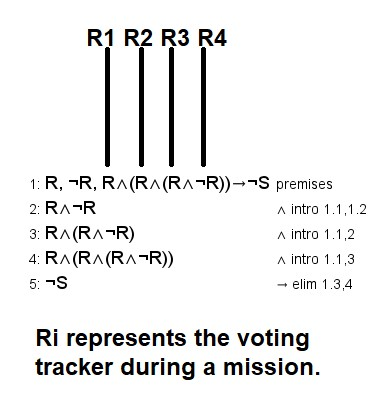
\includegraphics[scale=0.7]{im3.jpg}\newline
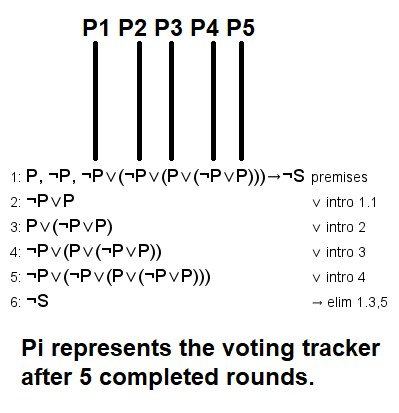
\includegraphics[scale=0.7]{im4.jpg}\newline
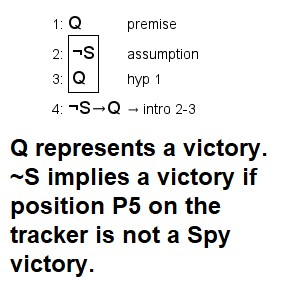
\includegraphics[scale=0.7]{im5.jpg}\newline

\section*{Model Exploration}
\addcontentsline{toc}{section}{Model Exploration}

When creating the model for the game, it  was unclear on  how to proceed with adding the constraints since the core of the game did not only depend on if the player played a Resistance token or Spy token but also factors such as vote tracker and round won had to be kept in mind.

In the initial stages of creating the encoding, there were only constraints for the token themselves. Such as mapping if R or S is true or false. However, as mentioned above this proved to be futile when taking into account other variables like vote tracking (Z). Whilst it was still necessary to maintain a mapping of the Resistance and Spy token; ultimately a better approach was to create constraints of the game condition itself per round. That way the model could be assessed based upon which missions were won or lost per game depending on what tokens were played and also if the mission was rejected via the vote tracker. \newline

For example: \newline

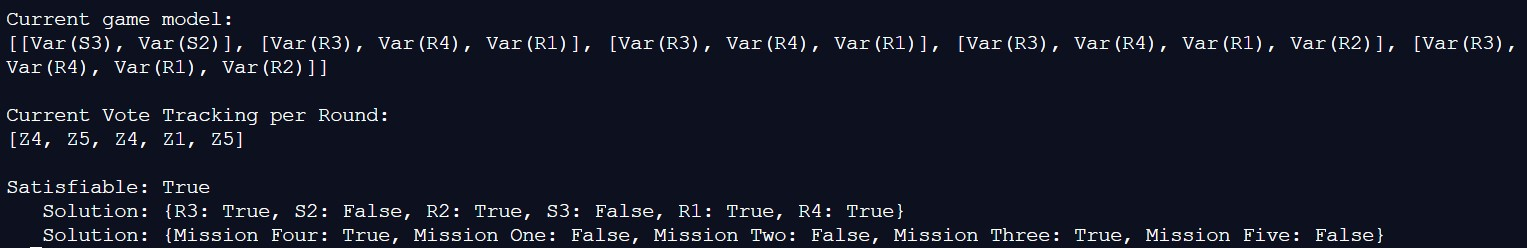
\includegraphics[scale=0.4, center]{scr3.jpg}\newline

In this case for mission two, it is clear that since there exists $R_1$ \& $R_2$ \& $R_3$, mission two should map out to true. However, as observed from the vote tracking, the second round’s mission was a failure as indicated by $Z_5$ in the vote tracker; therefore, mission two maps out to False rather than True.\newline

Additionally, a small alteration was done to assess if the model is satisfiable. Because of the nature of the constraints the models would continuously assess to true despite having a clear hypothesis that only certain models should map out to true if the game is won which occurs when the resistance wins 3 rounds. Therefore with the creation of a function called ResistanceWin() (which assesses if the resistance wins a game) and using that information conjoined with the is\_satisfiable() function was an alternative approach to examine if a model was satisfiable or not. \newline

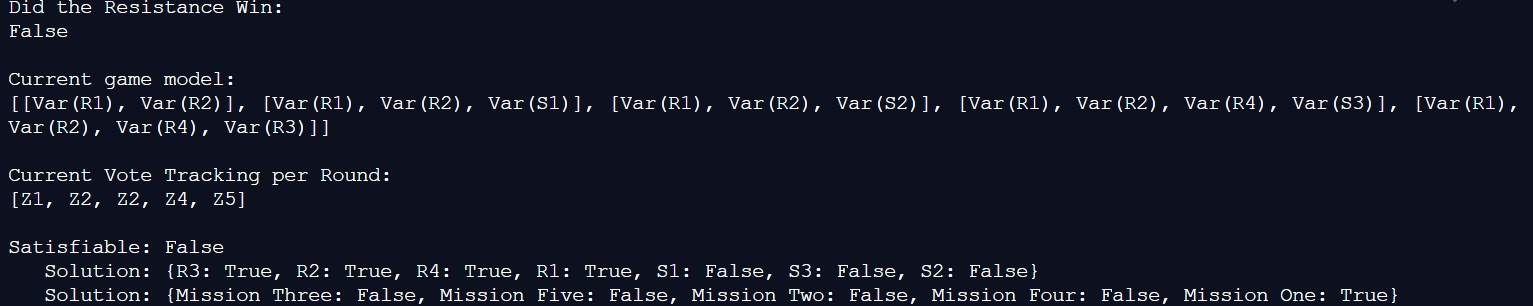
\includegraphics[scale=0.4, center]{scr4.jpg}\newline \newline \newline \newline 


After the likelihood function was implemented using the dsharp solver included with the given library, repeated tests were done to ensure that the output made sense. Initially a problem occurred: the probabilities were exclusively 1.0 or 0.0 – either the Resistance was guaranteed a cakewalk or devastating loss! This binary (pun intended) outcome was mystifying, but was eventually discovered to be caused by using the wrong variable in the denominator of the fraction. After a quick fix the probabilities were proven to be in the proper range of between 0 to 1.0 via several tests (shown below). Interestingly, the odds of team R winning never went above 50\% and were frequently below that, which indicates that according to our model the game is tilted in favour of the Spies. From this result it’s evident that the game is structured to keep naively honest players on their toes, although more real-life testing is required to verify this.\newline

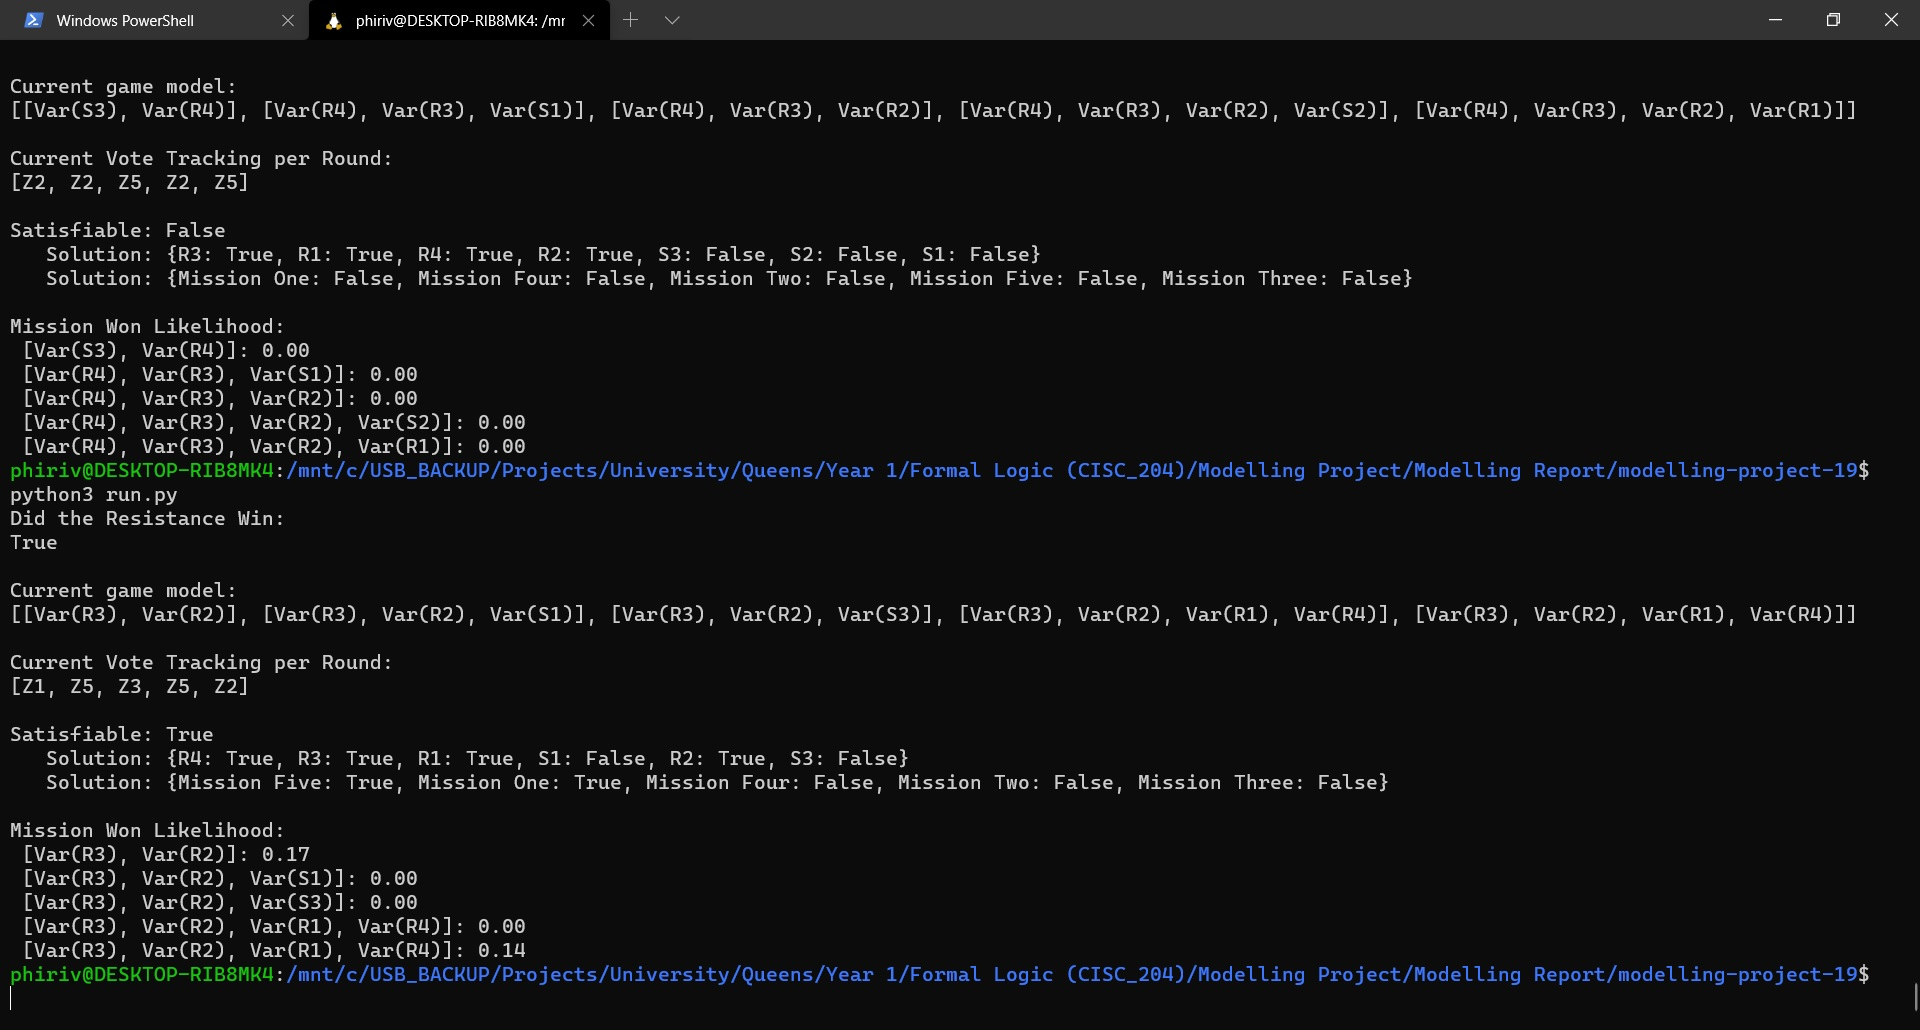
\includegraphics[scale=0.4, center]{scr1.jpg}\newline
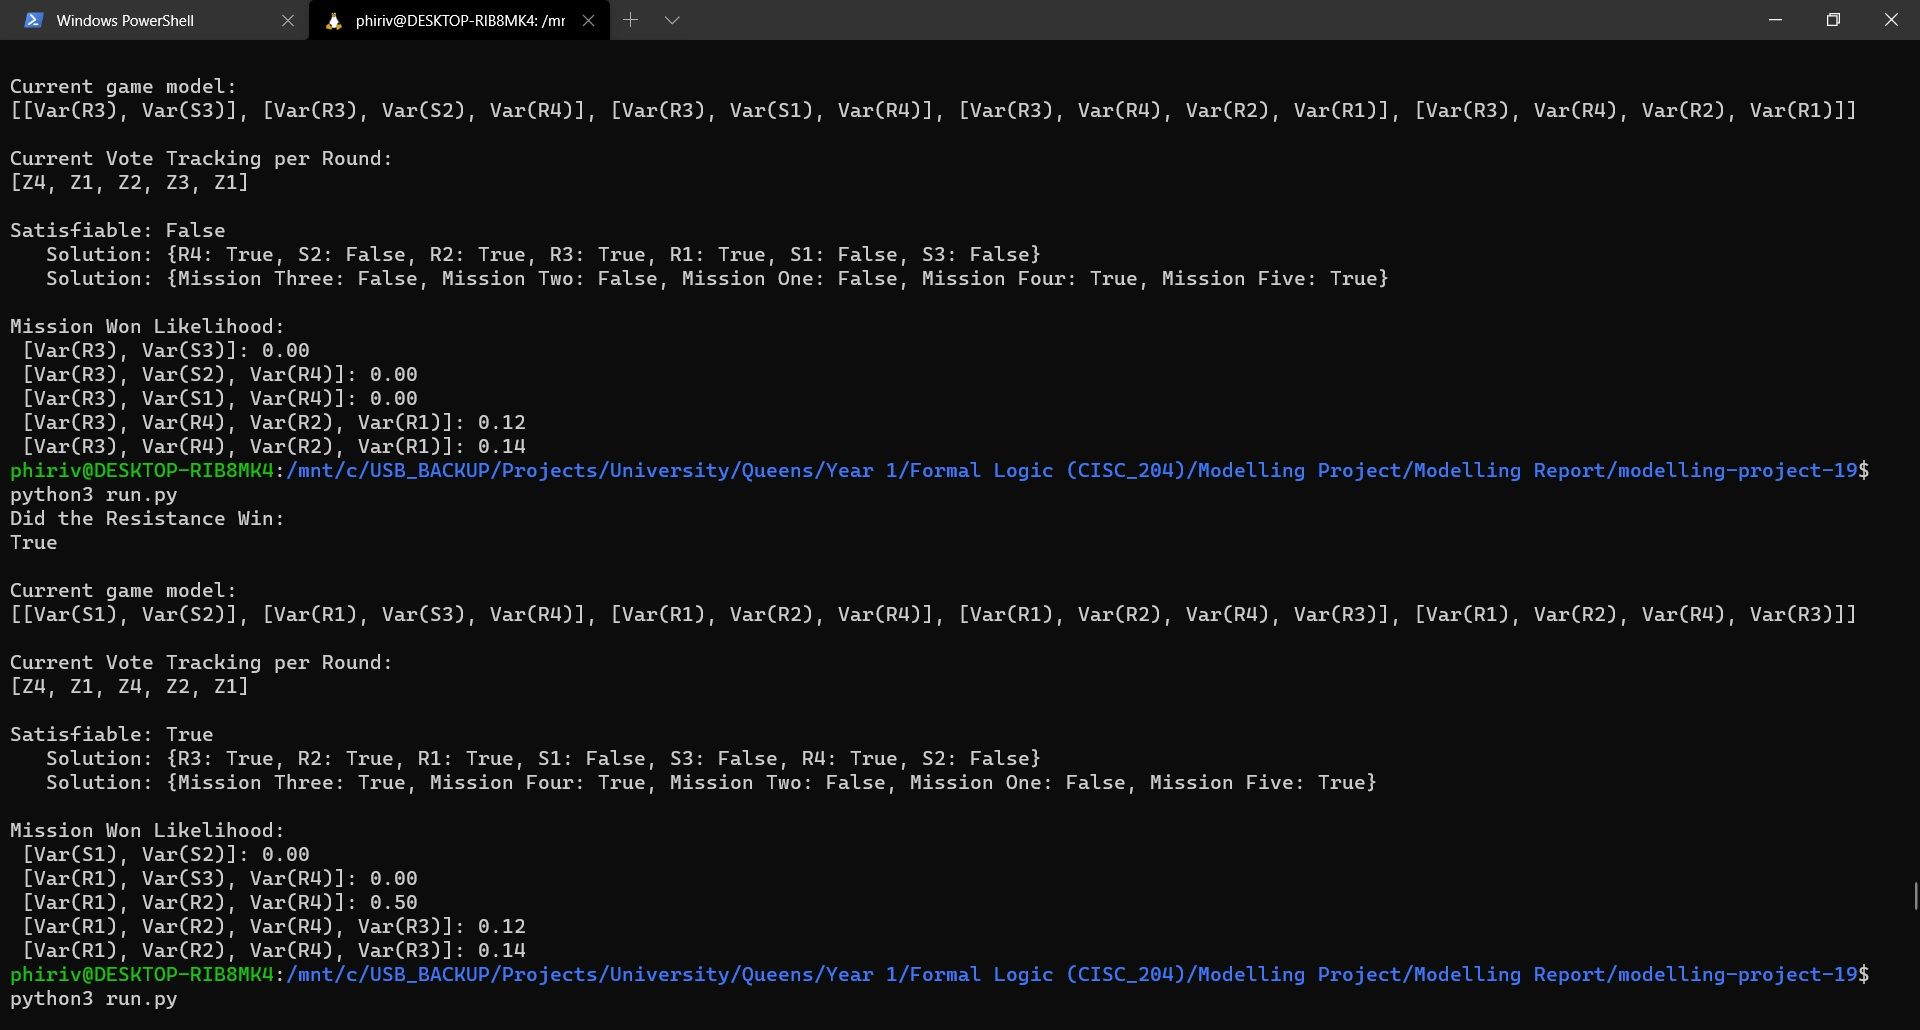
\includegraphics[scale=0.4, center]{scr2.jpg}\newline

Lastly, a final way the model was implemented was through a simple kind of automation. The various mission functions were coded so that (as per Prof. Muise's excellent advice), depending on what token was played the computer would make the most 'optimal' decision in choosing the team to go on the mission for the following rounds. This led to some interesting observations:\newline

\begin{enumerate}


	\item Since Mission Two and Mission Three have the same amount of tokens per their respective round, if the vote tracker for neither rounds is equal to $Z_5$, if Mission Two is true then in all cases Mission Three is true because the computer sends the same tokens from Mission Two onto Mission Three.
	\item If Mission One and Mission Two are false, the vote tracker for neither round is equal to $Z_5$ and tokens $S_1$, $S_2$ and $S_3$ are mapped to false then it is true for all cases that Mission Three, Four and Five are true, and as a result the Resistance wins the entire game. This is because the model has already identified the 3 spies prior; hence, there is a guaranteed win for the next three rounds.
	\item If Mission Five exists and Mission Four evaluates to true such that the vote tracker for round 4 is not equal to $Z_5$, it can be said that in all cases Mission Five will evaluate to true and the resistance will win the game. Hence, the model will be satisfiable and evaluates to true as well. This is because missions four and five contain the same number of player slots so the computer will automatically send all player tokens from Mission Four to Mission Five to guarantee a win for Mission Five. Additionally, the existence of Mission Five being true suggests that the game has not ended yet as none of the resistance or spy players have reached 3 points. Therefore, a guaranteed win for Mission Five (or evaluation to True) suggests that the Resistance are guaranteed to win the game and the model will be satisfiable. \newline

\end{enumerate}

%Describe how you might extend your model to a predicate logic setting, including how both the propositions and constraints would be updated. There is no need to implement this extension!
\section*{First Order Extension}
\addcontentsline{toc}{section}{First Order Extension}
Given the enumerative nature of our constraints in each voting round and mission, expanding the propositions to predicates is straightforward. \newline

For a rejection to occur the conjunctions involving $P_j$ are replaced with \indent$\forall x:P(x)$, where a single vote against is represented by $\exists x: \neg P(x)$. \newline \newline
\indent e.g. in round 1 ($i=1$):\newline
\indent$\exists i:X(i) \land \forall x:P(x) \rightarrow \exists i:Y(i)$\newline
\indent$\exists i:X(i) \land \exists x:\neg P(x) \rightarrow \exists i:\neg Y(i)$\newline

The 5 rejections in a row victory condition for the Spies directly follows:\newline
\indent$\forall y:Z(y) \rightarrow \forall k:\neg V(k)$\newline

After mission approval, a single $\exists z: \neg Q(z)$ representing a played fail token \indent causes the current mission to fail:\newline 
\indent$\exists i:Y(i)\land \exists z:\neg Q(z) \rightarrow \exists i:\neg S(i)$\newline

The final tally for the Resistance or Spies win condition is easily represented \indent with existential quantifiers:\newline
\indent$\exists a: \exists b: \exists c: S(a,b,c) \rightarrow \forall k:V(k)$\newline
\indent$\exists d: \exists e: \exists f: \neg S(d,e,f) \rightarrow \forall k:\neg V(k)$\newline

This radically simplifies things, as now it's no longer necessary to count every single different case where the Resistance wins 3 or more rounds to obtain an overall victory. Additional flexibility is gained for the possibility of increasing the number of rounds to an arbitrary number and subsequently changing the proportion of successes required for a given team to win the game.

\qed 

Thank you for taking the time to read this lengthy report! All the best

%\[ \wedge \hspace{4mm} \vee \hspace{4mm} \neg \hspace{4mm} \rightarrow \hspace{4mm} \forall \hspace{4mm} \exists \]


\end{document}
